        %%******************************************%%
        %%                                          %%
        %%        Modello di tesi di laurea         %%
        %%            di Andrea Giraldin            %%
        %%                                          %%
        %%             2 novembre 2012              %%
        %%                                          %%
        %%******************************************%%


% I seguenti commenti speciali impostano:
% 1. 
% 2. PDFLaTeX come motore di composizione;
% 3. tesi.tex come documento principale;
% 4. il controllo ortografico italiano per l'editor.

% !TEX encoding = UTF-8
% !TEX TS-program = pdflatex
% !TEX root = tesi.tex
% !TEX spellcheck = it-IT

\documentclass[10pt,                    % corpo del font principale
               a4paper,                 % carta A4
               twoside,                 % impagina per fronte-retro
               openright,               % inizio capitoli a destra
               english,                 
               italian,                 
               ]{book}    

\usepackage[utf8]{inputenc}             % codifica di input; anche [latin1] va bene
                                        % NOTA BENE! va accordata con le preferenze dell'editor

%**************************************************************
% Importazione package
%**************************************************************

%\usepackage{amsmath,amssymb,amsthm}    % matematica

\usepackage[english, italian]{babel}    % per scrivere in italiano e in inglese;
                                        % l'ultima lingua (l'italiano) risulta predefinita

\usepackage{bookmark}                   % segnalibri

\usepackage{caption}                    % didascalie

\usepackage{chngpage,calc}              % centra il frontespizio

\usepackage{csquotes}                   % gestisce automaticamente i caratteri (")

\usepackage{emptypage}                  % pagine vuote senza testatina e piede di pagina

\usepackage{epigraph}					% per epigrafi

\usepackage{eurosym}                    % simbolo dell'euro

\usepackage[T1]{fontenc}                % codifica dei font:
                                        % NOTA BENE! richiede una distribuzione *completa* di LaTeX

%\usepackage{indentfirst}               % rientra il primo paragrafo di ogni sezione

\usepackage{graphicx}                   % immagini

\usepackage{hyperref}                   % collegamenti ipertestuali



\usepackage[binding=5mm]{layaureo}      % margini ottimizzati per l'A4; rilegatura di 5 mm

\usepackage{listings}                   % codici

\usepackage{microtype}                  % microtipografia

\usepackage{mparhack,fixltx2e,relsize}  % finezze tipografiche

\usepackage{nameref}                    % visualizza nome dei riferimenti                                      

\usepackage[font=small]{quoting}        % citazioni

\usepackage{subfig}                     % sottofigure, sottotabelle

\usepackage[italian]{varioref}          % riferimenti completi della pagina

\usepackage[dvipsnames]{xcolor}         % colori

\usepackage{booktabs}                   % tabelle                                       
\usepackage{tabularx}                   % tabelle di larghezza prefissata                                    
\usepackage{longtable}                  % tabelle su più pagine
\usepackage{makecell,multirow}
\usepackage{placeins}
\usepackage{xcolor}
\usepackage{rotating}

\usepackage{ltxtable}                   % tabelle su più pagine e adattabili in larghezza

\usepackage[toc, acronym]{glossaries}   % glossario
                                        % per includerlo nel documento bisogna:
                                        % 1. compilare una prima volta tesi.tex;
                                        % 2. eseguire: makeindex -s tesi.ist -t tesi.glg -o tesi.gls tesi.glo
                                        % 3. eseguire: makeindex -s tesi.ist -t tesi.alg -o tesi.acr tesi.acn
                                        % 4. compilare due volte tesi.tex.
\usepackage[backend=biber,style=numeric-comp,citestyle=numeric-comp,hyperref,backref]{biblatex}
%\usepackage[backend=biber,style=verbose-ibid,hyperref,backref]{biblatex}
                                        % eccellente pacchetto per la bibliografia; 
                                        % produce uno stile di citazione autore-anno; 
                                        % lo stile "numeric-comp" produce riferimenti numerici
                                        % per includerlo nel documento bisogna:
                                        % 1. compilare una prima volta tesi.tex;
                                        % 2. eseguire: biber tesi
                                        % 3. compilare ancora tesi.tex.

%**************************************************************
% file contenente le impostazioni della tesi
%**************************************************************

%**************************************************************
% Frontespizio
%**************************************************************

\definecolor{verde}{rgb}{0.0, 0.5, 0.0}
% Autore
\newcommand{\myName}{Beatrice Liberi}                                    
\newcommand{\myTitle}{Analisi e Implementazione di Algoritmi per problemi di Scheduling}

%Azienda
\newcommand{\TS}{Trans-Cel Autotrasporti}
\newcommand{\task}{\textit{Task}}
\newcommand{\items}{\textit{Item}}
\newcommand{\ttb}{\textit{TTB}}

% Tipo di tesi                   
\newcommand{\myDegree}{Tesi di laurea triennale}

% Università             
\newcommand{\myUni}{Università degli Studi di Padova}

% Facoltà       
\newcommand{\myFaculty}{Corso di Laurea in Informatica}

% Dipartimento
\newcommand{\myDepartment}{Dipartimento di Matematica "Tullio Levi-Civita"}

% Titolo del relatore
\newcommand{\profTitle}{Prof.}

% Relatore
\newcommand{\myProf}{Luigi De Giovanni}

% Luogo
\newcommand{\myLocation}{Padova}

% Anno accademico
\newcommand{\myAA}{2016-2017}

% Data discussione
\newcommand{\myTime}{Settembre 2017}


%**************************************************************
% Impostazioni di impaginazione
% see: http://wwwcdf.pd.infn.it/AppuntiLinux/a2547.htm
%**************************************************************

\setlength{\parindent}{14pt}   % larghezza rientro della prima riga
\setlength{\parskip}{0pt}   % distanza tra i paragrafi

\newlength{\offsetpage}
\setlength{\offsetpage}{1.0cm}
\newenvironment{widepage}
    {\begin{adjustwidth}{-\offsetpage}{-\offsetpage}%
        \addtolength{\textwidth}{2\offsetpage}}%
    {\end{adjustwidth}}

%**************************************************************
% Impostazioni di biblatex
%**************************************************************
\bibliography{bibliografia} % database di biblatex 

\defbibheading{bibliography} {
    \cleardoublepage
    \phantomsection 
    \addcontentsline{toc}{chapter}{\bibname}
    \chapter*{\bibname\markboth{\bibname}{\bibname}}
}

\setlength\bibitemsep{1.5\itemsep} % spazio tra entry

\DeclareBibliographyCategory{opere}
\DeclareBibliographyCategory{web}

\addtocategory{opere}{womak:lean-thinking}
\addtocategory{web}{site:agile-manifesto}

\defbibheading{opere}{\section*{Riferimenti bibliografici}}
\defbibheading{web}{\section*{Siti Web consultati}}


%**************************************************************
% Impostazioni di caption
%**************************************************************
\captionsetup{
    tableposition=top,
    figureposition=bottom,
    font=small,
    format=hang,
    labelfont=bf
}

%**************************************************************
% Impostazioni di glossaries
%**************************************************************

%**************************************************************
% Acronimi
%**************************************************************
\renewcommand{\acronymname}{Acronimi e abbreviazioni}

\newacronym{uml}{UML}{Unified Modeling Language}

\newacronym{ampl}{AMPL}{A Mathematical Programming Language}

\newacronym{ide}{IDE}{Integrated Developement Environment}

%**************************************************************
% Glossario
%**************************************************************
\renewcommand{\glossaryname}{Glossario}

\newglossaryentry{umlg}
{
    name=\glslink{uml}{UML},
    text=UML,
    sort=uml,
    description={in ingegneria del software \emph{UML, Unified Modeling Language} (ing. linguaggio di modellazione unificato) è un linguaggio di modellazione e specifica basato sul paradigma object-oriented. L'\emph{UML} svolge un'importantissima funzione di ``lingua franca'' nella comunità della progettazione e programmazione a oggetti. Gran parte della letteratura di settore usa tale linguaggio per descrivere soluzioni analitiche e progettuali in modo sintetico e comprensibile a un vasto pubblico}
}

\newglossaryentry{probsched}
{
    name=Problema di Schedulazione/Scheduling,
    text=problemi di scheduling,
    sort=problemi di scheduling,
    description={Un problema di schedulazione definisce le variabili decisionali, una regione ammissibile entro la quale le variabili decisionali possono variare e una funzione obiettivo per determinare la migliore \emph{\gls{sched}}\glsfirstoccur\ ammissibile}
}

\newglossaryentry{sched}
{
    name=Schedulazione/Scheduling,
    text=schedulazione,
    sort=schedulazione,
    description={La schedulazione è una forma di processo decisionale che consiste nell'allocare risorse finite in modo tale che un dato obiettivo venga ottimizzato, sincronizzando e tempificando la sequenza delle operazioni}
}

\newglossaryentry{metodo-esatto}
{
    name=Metodo esatto,
    text=metodo esatto,
    sort=metodo esatto,
    description={I metodi di risoluzione dei problemi di ottimizzazione combinatoria ricadono in due categorie: i metodi esatti e metodi euristici (vd. \textit{Algoritmo euristico}). I primi sono metodi che riescono a fornire una soluzione ottima, a differenza dei secondi che riescono a fornire una soluzione ammissibile ma senza la garanzia che sia ottimale.\footcite{degio:dispensa}
    Esempi di algoritmi esatti sono il simplesso o il branch-and-bound}
}

\newglossaryentry{algeur}
{
    name=Algoritmo euristico,
    text=euristici,
    sort=algoritmo euristico,
    description={I metodi di risoluzione dei problemi di ottimizzazione combinatoria ricadono in due categorie: i metodi esatti (vd. \textit{Metodo esatto}) e metodi euristici. In matematica e informatica un metodo euristico è un particolare tipo di algoritmo progettato per risolvere un problema di ricerca operativa più velocemente (qualora i metodi esatti siano troppo lenti) o per trovare una soluzione approssimata (qualora i metodi esatti falliscano nel trovare una soluzione esatta). Il risultato viene ottenuto cercando di equilibrare ottimalità, completezza, accuratezza e velocità di esecuzione. \\
    Possono essere applicati quando la soluzione è data selezionando il miglior sottoinsieme di un dato insieme di elementi e sono costruttivi, ovvero partono da una soluzione vuota e ad ogni iterazione aggiungono un elemento applicando dei criteri di selezione\footcite{degio:dispensa}}
}

\newglossaryentry{greedy}
{
    name=Algoritmo Greedy,
    text=greedy,
    sort=algoritmo greedy,
    description={Un algoritmo greedy è un algoritmo euristico che ad ogni iterazione compie una scelta ``golosa'', ovvero la migliore (in termini di impatto sulla funzione obiettivo) da prendere in quel momento}
}

\newglossaryentry{meteur}
{
    name=Meta-euristica,
    text=meta-euristici,
    sort=meta-euristica,
    description={In matematica e informatica è una strategia per esplorare in maniera efficiente lo spazio delle soluzioni per trovare delle soluzioni vicine all'ottimo e scappare dagli ottimi locali. Non sono algoritmi costruttivi e necessitano quindi di una soluzione per poterne trovarne un'altra migliore}
}

\newglossaryentry{tabu}
{
    name=Tabu Search,
    text=Tabu Search,
    sort=Tabu Search,
    description={La Tabu Search è una tecnica meta-euristica utilizzata per la soluzione di numerosi problemi di ottimizzazione, tra cui problemi di scheduling. Essa consiste nel partire da una soluzione iniziale ed eseguire una serie di ``mosse'' che portano ad una nuova soluzione all'interno del vicinato per la quale la funzione obiettivo f assume un valore migliore del valore attuale. Per sfuggire gli ottimi locali, la Tabu Search permette un certo numero di mosse peggioranti rendendo tabù, proibite, le ultime mosse eseguite per evitare di ``tornare indietro''}
}

\newglossaryentry{supply-chain}
{
    name=Supply chain,
    text=supply chain,
    sort=supply chain,
    description={La supply chain (in italiano, ``catena di distribuzione'') è il sistema di organizzazioni, persone, attività, informazioni e risorse coinvolte nel portare un prodotto o un servizio dal fornitore al cliente}
}

\newglossaryentry{dummy}
{
    name=Dummy worker,
    text=Dummy Worker,
    sort=dummy worker,
    description={Nel campo degli algoritmi euristici e dei problemi di scheduling, aggiungere un Dummy Worker è una tecnica usata per produrre sempre una soluzione ammissibile, anche quando in realtà l'algoritmo euristico non riesce a trovarne una. Il Dummy Worker può essere assegnato senza alcun vincolo a qualsiasi \task\ durante qualsiasi \ttb, tuttavia inserirlo introduce una penalità altissima per la funzione obiettivo, di conseguenza viene introdotto in uno scheduling quando non c'è nessun'altra alternativa. Nello scheduling finale, il numero di \task\ non assegnati corrisponde al numero di \task\ assegnati al Dummy Worker\\}
}


\newglossaryentry{nphard}
{
    name=NP-Hard,
    text=NP-Hard,
    sort=nphard,
    description={vd. \emph{\gls{teoria-compl}}\glsfirstoccur}
}

\newglossaryentry{teoria-compl}
{
    name=Teoria della complessità computazionale,
    text=teoria della complessità computazionale,
    sort=teoria,
    description={In informatica, la teoria della complessità computazionale è una branca della teoria della computabilità che studia le risorse minime necessarie (principalmente tempo di calcolo e memoria) per la risoluzione di un problema. I problemi sono classificati in differenti classi di complessità, in base all'efficienza del migliore algoritmo noto in grado di risolvere quello specifico problema:
    \begin{itemize}
        \item $\mathcal{P}$ (\textit{Polynomial-time problems}) - Contiene tutti i problemi decisionali che possono essere risolti da una macchina di Turing deterministica in tempo polinomiale. La classe $\mathcal{P}$ può essere caratterizzata come quella classe di problemi per i quali si è in grado di trovare una soluzione in tempo polinomiale.
        \item $\mathcal{NP}$ (\textit{Nondeterministic polynomial-time problems}) - Contiene tutti i problemi decisionali che possono essere risolti da una macchina di Turing non deterministica in tempo polinomiale. La classe $\mathcal{NP}$ può essere caratterizzata come quella classe di problemi per i quali non si è in grado di trovare una soluzione in tempo polinomiale, ma si è in grado di verificare se una possibile soluzione è effettivamente tale in tempo polinomiale. \\ In particolare, $\mathcal{P} \subseteq\ \mathcal{NP}$.
        \item $\mathcal{NP-C}$ o NP-Completi - Sono i più difficili problemi nella classe $\mathcal{NP}$: se si trovasse un algoritmo in grado di risolvere in tempo polinomiale un qualsiasi problema in $\mathcal{NP-C}$, allora si potrebbe usarlo per risolvere in tempo polinomiale ogni problema in $\mathcal{NP}$. \\ In particolare, $\mathcal{NP-C} \subseteq\ \mathcal{NP}$.
        \item $\mathcal{H}$ o NP-Hard (\textit{Nondeterministic polynomial-time hard problems}) -  Classe di problemi (non limitata ai soli problemi di decisione, ma estesa anche ai problemi di ottimizzazione, ad esempio) che può essere definita informalmente come la classe dei problemi non meno difficili dei problemi $\mathcal{NP-C}$, che a loro volta sono per definizione i più difficili della classe $\mathcal{NP}$. Si noti che non è sempre vero che $\mathcal{H} \subseteq\ \mathcal{NP}$.
    \end{itemize}
    (\cite{wiki:teoria-compl}.)
    }
}

\newglossaryentry{framework}
{
    name=Framework,
    text=framework,
    sort=framework,
    description={Nello sviluppo software, il framework è un'architettura logica di supporto su cui un software può essere progettato e realizzato; la sua funzione è quella di creare una infrastruttura generale, lasciando al programmatore il contenuto vero e proprio dell'applicazione}
}

\newglossaryentry{amplg}
{
    name=\gls{ampl},
    text=AMPL,
    sort=ampl,
    description={È un linguaggio ad alto livello per descrivere e risolvere grossi e complicati problemi di programmazione matematica (per esempio problemi di ottimizzazione e di scheduling)}
}

\newglossaryentry{ideg}
{
    name=\gls{ide},
    text=IDE,
    sort=ide,
    description={È un software che, in fase di programmazione, aiuta il programmatore nello sviluppo del codice sorgente fornendo un controllo sintassi in tempo reale e una serie di strumenti e funzionalità di supporto allo sviluppo e al debugging}
}

\newglossaryentry{drive}
{
    name=Google Drive,
    text=Google Drive,
    sort=google drive,
    description={Servizio fornito da Google in ambiente cloud computing che offre funzioni di condivisione e hosting di file, permettendone la modifica collaborativa su uno spazio gratuito di 15 GB}
}

\newglossaryentry{repository}
{
    name=Repository,
    text=repository,
    sort=repository,
    description={Ambiente di un sistema informativo in cui vengono gestiti i metadati attraverso tabelle relazionali. L'insieme di tabelle, regole e motori di calcolo tramite cui si gestiscono i metadati prende il nome di metabase}
}

\newglossaryentry{git}
{
    name=Git,
    text=Git,
    sort=git,
    description={Software di controllo versione distribuito utilizzabile da interfaccia a riga di comando. È uno dei pù diffusi strumenti di controllo versione}
}

\newglossaryentry{mod-incr}
{
    name=Modello incrementale,
    text=modello incrementale,
    sort=modello incrementale,
    description={In ingegneria del software, è una metodologia di sviluppo software in cui il cliente identifica, a grandi linee, i requisiti fondamentali e quelli desiderabili del prodotto software che vuole ottenere; viene poi deciso il numero di incrementi da effettuare, tenendo conto del fatto che ogni singolo incremento costituisce un sottoinsieme delle funzionalità del prodotto software. Una volta che gli incrementi sono stati identificati, si definiscono in dettaglio i requisiti che devono essere soddisfatti dagli incrementi prima di procedere allo sviluppo}
}

\newglossaryentry{agile}
{
    name=Agile,
    text=agile,
    sort=agile,
    description={In ingegneria del software, è un insieme di metodi di sviluppo del software emersi a partire dai primi anni 2000 e fondati su insieme di principi comuni, direttamente o indirettamente derivati dai principi del ``Manifesto per lo sviluppo agile del software''\footcite{manifesto}. Tale manifesto si può riassumere in quattro punti:
        \begin{enumerate}
            \item le persone e le interazioni sono più importanti dei processi e degli strumenti;
            \item è più importante avere software funzionante che documentazione;
            \item bisogna collaborare con i clienti oltre che rispettare il contratto;
            \item bisogna essere pronti a rispondere ai cambiamenti oltre che aderire alla pianificazione.
        \end{enumerate}
    Un esempio di metodo di sviluppo di tipo agile è il metodo \emph{\gls{scrum}}\glsfirstoccur}
}

\newglossaryentry{scrum}
{
    name=Scrum,
    text=scrum,
    sort=scrum,
    description={Metodo di sviluppo software che rientra fra i metodi agile. Prevede di dividere il progetto in blocchi rapidi di lavoro (Sprint) alla fine di ciascuno dei quali creare un incremento del software. Esso indica come definire i dettagli del lavoro da fare nell'immediato futuro e prevede vari meeting con caratteristiche precise per creare occasioni di ispezione e controllo del lavoro svolto}
}

\newglossaryentry{milestone}
{
    name=Milestone,
    text=milestones,
    sort=milestone,
    description={Traguardi intermedi ed importanti nello svolgimento di un progetto; sono spesso fissati in fase di pianificazione}
}

\newglossaryentry{gantt}
{
    name=Diagramma di Gantt,
    text=,
    sort=diagramma,
    description={Tipo di diagrammi molto usato per le attività di amministrazione di progetti poiché
        permettono una rappresentazione visuale di facile comprensione della durata delle attività
        che verranno svolte e le loro dipendenze. I Diagrammi di Gantt sono molto importanti
        per la gestione delle risorse di un progetto e per la creazione di un calendario delle attività
        che sia efficace}
}

\newglossaryentry{bus-logic}
{
    name=Business logic,
    text=business logic,
    sort=business logic,
    description={L'espressione logica di business (en. \textit{business logic}) si riferisce a tutta la logica applicativa che rende operativa un'applicazione. Con tale nome ci si riferisce quindi all'algoritmica che gestisce lo scambio di informazioni tra una sorgente dati e l'interfaccia utente attraverso la logica di presentazione e le elaborazioni intermedie sui dati estratti.
}}

\newglossaryentry{arch-ntier}
{
    name=Architettura multi-tier,
    text=architettura multi-tier,
    sort=architettura multi-tier,
    description={In ingegneria del software, indica un'architettura software in cui le varie funzionalità del software sono logicamente separate e suddivise in più strati (\textit{tier}) in comunicazione fra loro. L'impiego più diffuso di un'architettura multi-tier è l'\emph{\gls{arch-3tier}}\glsfirstoccur   
}}

\newglossaryentry{arch-3tier}
{
    name=Architettura three-tier,
    text=architettura three-tier,
    sort=architettura three-tier,
    description={Questa architettura software è costruita su tre livelli:
        \begin{itemize}
            \item livello di presentazione: è il livello più alto, 
            \item livello applicazione, o \textit{business logic}:
            \item livello dati:
        \end{itemize}
}}

\newglossaryentry{design}
{
    name=Design pattern,
    text=design pattern,
    sort=design,
    description={In informatica, per Design Pattern si intende un modello logico che rappresenta una soluzione progettuale generale ad un problema ricorrente. Durante le fasi di progettazione del software può essere utile applicare uno di questi modelli logici per risolvere un particolare problema che può presentarsi in più di una situazione.
}}


 % database di termini
\makeglossaries


%**************************************************************
% Impostazioni di graphicx
%**************************************************************
\graphicspath{{immagini/}} % cartella dove sono riposte le immagini


%**************************************************************
% Impostazioni di hyperref
%**************************************************************
\hypersetup{
    %hyperfootnotes=false,
    %pdfpagelabels,
    %draft,	% = elimina tutti i link (utile per stampe in bianco e nero)
    colorlinks=true,
    linktocpage=true,
    pdfstartpage=1,
    pdfstartview=FitV,
    % decommenta la riga seguente per avere link in nero (per esempio per la stampa in bianco e nero)
    %colorlinks=false, linktocpage=false, pdfborder={0 0 0}, pdfstartpage=1, pdfstartview=FitV,
    breaklinks=true,
    pdfpagemode=UseNone,
    pageanchor=true,
    pdfpagemode=UseOutlines,
    plainpages=false,
    bookmarksnumbered,
    bookmarksopen=true,
    bookmarksopenlevel=1,
    hypertexnames=true,
    pdfhighlight=/O,
    %nesting=true,
    %frenchlinks,
    urlcolor=webbrown,
    linkcolor=RoyalBlue,
    citecolor=webgreen,
    %pagecolor=RoyalBlue,
    %urlcolor=Black, linkcolor=Black, citecolor=Black, %pagecolor=Black,
    pdftitle={\myTitle},
    pdfauthor={\textcopyright\ \myName, \myUni, \myFaculty},
    pdfsubject={},
    pdfkeywords={},
    pdfcreator={pdfLaTeX},
    pdfproducer={LaTeX}
}

%**************************************************************
% Impostazioni di itemize
%**************************************************************
\renewcommand{\labelitemi}{$\ast$}

%\renewcommand{\labelitemi}{$\bullet$}
%\renewcommand{\labelitemii}{$\cdot$}
%\renewcommand{\labelitemiii}{$\diamond$}
%\renewcommand{\labelitemiv}{$\ast$}


%**************************************************************
% Impostazioni di listings
%**************************************************************
\lstset{
    language=[LaTeX]Tex,%C++,
    keywordstyle=\color{RoyalBlue}, %\bfseries,
    basicstyle=\small\ttfamily,
    %identifierstyle=\color{NavyBlue},
    commentstyle=\color{Green}\ttfamily,
    stringstyle=\rmfamily,
    numbers=none, %left,%
    numberstyle=\scriptsize, %\tiny
    stepnumber=5,
    numbersep=8pt,
    showstringspaces=false,
    breaklines=true,
    frameround=ftff,
    frame=single
} 


%**************************************************************
% Impostazioni di xcolor
%**************************************************************
\definecolor{webgreen}{rgb}{0,.5,0}
\definecolor{webbrown}{rgb}{.6,0,0}


%**************************************************************
% Altro
%**************************************************************

\newcommand{\omissis}{[\dots\negthinspace]} % produce [...]

% eccezioni all'algoritmo di sillabazione
\hyphenation
{
    ma-cro-istru-zio-ne
    gi-ral-din
}

\newcommand{\sectionname}{sezione}
\addto\captionsitalian{\renewcommand{\figurename}{Figura}
                       \renewcommand{\tablename}{Tabella}}

\newcommand{\glsfirstoccur}{\ap{{[g]}}}

\newcommand{\intro}[1]{\emph{\textsf{#1}}}

%**************************************************************
% Environment per ``rischi''
%**************************************************************
\newcounter{riskcounter}                % define a counter
\setcounter{riskcounter}{0}             % set the counter to some initial value

%%%% Parameters
% #1: Title
\newenvironment{risk}[1]{
    \refstepcounter{riskcounter}        % increment counter
    \par \noindent                      % start new paragraph
    \textbf{\arabic{riskcounter}. #1}   % display the title before the 
                                        % content of the environment is displayed 
}{
    \par\medskip
}

\newcommand{\riskname}{Rischio}

\newcommand{\riskdescription}[1]{\textbf{\\Descrizione:} #1.}

\newcommand{\risksolution}[1]{\textbf{\\Soluzione:} #1.}

%**************************************************************
% Environment per ``use case''
%**************************************************************
\newcounter{usecasecounter}             % define a counter
\setcounter{usecasecounter}{0}          % set the counter to some initial value

%%%% Parameters
% #1: ID
% #2: Nome
\newenvironment{usecase}[2]{
    \renewcommand{\theusecasecounter}{\usecasename #1}  % this is where the display of 
                                                        % the counter is overwritten/modified
    \refstepcounter{usecasecounter}             % increment counter
    \vspace{10pt}
    \par \noindent                              % start new paragraph
    {\large \textbf{\usecasename #1: #2}}       % display the title before the 
                                                % content of the environment is displayed 
    \medskip
}{
    \medskip
}

\newcommand{\usecasename}{UC}

\newcommand{\usecaseactors}[1]{\textbf{\\Attori Principali:} #1. \vspace{4pt}}
\newcommand{\usecasepre}[1]{\textbf{\\Precondizioni:} #1. \vspace{4pt}}
\newcommand{\usecasedesc}[1]{\textbf{\\Descrizione:} #1. \vspace{4pt}}
\newcommand{\usecasepost}[1]{\textbf{\\Postcondizioni:} #1. \vspace{4pt}}
\newcommand{\usecasealt}[1]{\textbf{\\Scenario Alternativo:} #1. \vspace{4pt}}

%**************************************************************
% Environment per ``namespace description''
%**************************************************************

\newenvironment{namespacedesc}{
    \vspace{10pt}
    \par \noindent                              % start new paragraph
    \begin{description} 
}{
    \end{description}
    \medskip
}

\newcommand{\classdesc}[2]{\item[\textbf{#1:}] #2}

%****************************************************************
%Scrittura di codice
%****************************************************************
\usepackage{listings}
\usepackage{color}

\definecolor{dkgreen}{rgb}{0,0.6,0}
\definecolor{gray}{rgb}{0.5,0.5,0.5}
\definecolor{mauve}{rgb}{0.58,0,0.82}

\lstset{frame=tb,
    language=C,
    aboveskip=3mm,
    belowskip=3mm,
    showstringspaces=false,
    columns=flexible,
    basicstyle={\small\ttfamily},
    numbers=none,
    numberstyle=\tiny\color{gray},
    keywordstyle=\color{blue},
    commentstyle=\color{dkgreen},
    stringstyle=\color{mauve},
    breaklines=true,
    breakatwhitespace=true,
    tabsize=3,
    % new keywords color
    classoffset=1,
    morekeywords={preprocessCandidates},
    keywordstyle=\color{WildStrawberry},
    classoffset=2,
    morekeywords={filterCandidate},
    keywordstyle=\color{WildStrawberry},
    classoffset=3,
    morekeywords={stopConditions},
    keywordstyle=\color{WildStrawberry},
    classoffset=4,
    morekeywords={ifCandidateFound},
    keywordstyle=\color{WildStrawberry},
    classoffset=5,
    morekeywords={isFeasible},
    keywordstyle=\color{WildStrawberry},
    classoffset=6,
    morekeywords={UNFEASIBLE},
    keywordstyle=\color{dkgreen},
    classoffset=7,
    morekeywords={SUCCESS_RUN},
    keywordstyle=\color{dkgreen},
    classoffset=0% restore to default class if more customisations...
}                     % file con le impostazioni personali

\begin{document}
%**************************************************************
% Materiale iniziale
%**************************************************************
\frontmatter
% !TEX encoding = UTF-8
% !TEX TS-program = pdflatex
% !TEX root = ../tesi.tex

%**************************************************************
% Frontespizio 
%**************************************************************
\begin{titlepage}

\begin{center}

\begin{LARGE}
\textbf{\myUni}\\
\end{LARGE}

\vspace{10pt}

\begin{Large}
\textsc{\myDepartment}\\
\end{Large}

\vspace{10pt}

\begin{large}
\textsc{\myFaculty}\\
\end{large}

\vspace{30pt}
\begin{figure}[htbp]
\begin{center}

\includegraphics[height=6cm]{logo-unipd}
\end{center}
\end{figure}
\vspace{30pt} 

\begin{LARGE}
\begin{center}
\textbf{\myTitle}\\
\end{center}
\end{LARGE}

\vspace{10pt} 

\begin{large}
\textsl{\myDegree}\\
\end{large}

\vspace{40pt} 

\begin{large}
\begin{flushleft}
\textit{Relatore}\\ 
\vspace{5pt} 
\profTitle\ \myProf
\end{flushleft}

\vspace{0pt} 

\begin{flushright}
\textit{Laureanda}\\ 
\vspace{5pt} 
\myName
\end{flushright}
\end{large}

\vspace{40pt}

\line(1, 0){338} \\
\begin{normalsize}
\textsc{Anno Accademico \myAA}
\end{normalsize}

\end{center}
\end{titlepage} 
% !TEX encoding = UTF-8
% !TEX TS-program = pdflatex
% !TEX root = ../tesi.tex

%**************************************************************
% Colophon
%**************************************************************
\clearpage
\phantomsection
\thispagestyle{empty}

\hfill

\vfill

\noindent\myName: \textit{\myTitle,}
\myDegree,
\textcopyright\ \myTime.
%% !TEX encoding = UTF-8
% !TEX TS-program = pdflatex
% !TEX root = ../tesi.tex

%**************************************************************
% Dedica
%**************************************************************
\cleardoublepage
\phantomsection
\thispagestyle{empty}
\pdfbookmark{Dedica}{Dedica}

\vspace*{3cm}

\begin{center}
Più si allarga l'isola della conoscenza, più si allunga il confine del mistero.\\ \medskip
--- John A. Wheeler 
\end{center}


% !TEX encoding = UTF-8
% !TEX TS-program = pdflatex
% !TEX root = ../tesi.tex

%**************************************************************
% Sommario
%**************************************************************
\cleardoublepage
\phantomsection
\pdfbookmark{Sommario}{Sommario}
\begingroup
\let\clearpage\relax
\let\cleardoublepage\relax
\let\cleardoublepage\relax

\chapter*{Sommario}

Il presente documento descrive il lavoro che ho svolto durante il periodo di stage, della durata di trecento ore, presso l'azienda \TS. \\ \\
Lo scopo dello stage è stato lo studio di modelli per problemi di scheduling e l'implementazione di algoritmi euristici che restituiscano una soluzione ammissibile in tempi sufficientemente brevi per una pianificazione in tempo reale. Il progetto ha fornito a \TS\ uno strumento che potrà essere integrato nei software di pianificazion sviluppati in azienda e da applicare in diversi contesti per i quali sia necessaria la risoluzione di un problema di scheduling. \\ \\
Gli obiettivi da raggiungere nel corso dello stage erano molteplici: 
in primo luogo era richiesto di assimilare i concetti di base dei problemi di scheduling, studiare la letteratura scientifica sui modelli e sugli algoritmi euristici più adatti per risolvere gli stessi; in secondo luogo era richiesto di definire formalmente con un modello matematico un problema di scheduling da risolvere, e progettare un algoritmo euristico per trovare una soluzione al problema; terzo ed ultimo obiettivo era l'implementazione dell'algoritmo euristico, integrandolo nelle librerie dell'azienda.

\endgroup			

\vfill


% !TEX encoding = UTF-8
% !TEX TS-program = pdflatex
% !TEX root = ../tesi.tex

%**************************************************************
% Ringraziamenti
%**************************************************************
\cleardoublepage
\phantomsection
\pdfbookmark{Ringraziamenti}{ringraziamenti}

\begin{flushright}{
	\slshape    
	``Life is really simple, but we insist on making it complicated''} \\ 
	\medskip
    --- Confucius
\end{flushright}


\bigskip

\begingroup
\let\clearpage\relax
\let\cleardoublepage\relax
\let\cleardoublepage\relax

\chapter*{Ringraziamenti}

\noindent \textit{Innanzitutto, vorrei esprimere la mia gratitudine al Prof. NomeDelProfessore, relatore della mia tesi, per l'aiuto e il sostegno fornitomi durante la stesura del lavoro.}\\

\noindent \textit{Desidero ringraziare con affetto i miei genitori per il sostegno, il grande aiuto e per essermi stati vicini in ogni momento durante gli anni di studio.}\\

\noindent \textit{Ho desiderio di ringraziare poi i miei amici per tutti i bellissimi anni passati insieme e le mille avventure vissute.}\\
\bigskip

\noindent\textit{\myLocation, \myTime}
\hfill \myName

\endgroup


% !TEX encoding = UTF-8
% !TEX TS-program = pdflatex
% !TEX root = ../tesi.tex

%**************************************************************
% Indici
%**************************************************************
\cleardoublepage
\pdfbookmark{\contentsname}{tableofcontents}
\setcounter{tocdepth}{2}
\tableofcontents
%\markboth{\contentsname}{\contentsname} 
\clearpage

\begingroup 
    \let\clearpage\relax
    \let\cleardoublepage\relax
    \let\cleardoublepage\relax
    %*******************************************************
    % Elenco delle figure
    %*******************************************************    
    \phantomsection
    \pdfbookmark{\listfigurename}{lof}
    \listoffigures

    \vspace*{8ex}
    %*******************************************************
    % Elenco delle tabelle
    %*******************************************************
    \newpage
    \phantomsection
    \pdfbookmark{\listtablename}{lot}
    \listoftables
        
    \vspace*{8ex}
\endgroup

\cleardoublepage

\cleardoublepage

%**************************************************************
% Materiale principale
%**************************************************************
\mainmatter
% !TEX encoding = UTF-8
% !TEX TS-program = pdflatex
% !TEX root = ../tesi.tex

%**************************************************************
\chapter{Introduzione}
\label{cap:introduzione}
%**************************************************************

\intro{In questo capitolo vengono brevemente descritte l'azienda \TS\ presso la quale ho svolto lo stage e l'idea dalla quale è nata la necessità del progetto portato a termine durante lo stesso. \\
Viene inoltre presentata la suddivisione della tesi per capitoli e vengono introdotte alcune norme tipografiche che verranno utilizzate di seguito.}

%**************************************************************
\section{L'azienda}

\TS\ è un'azienda che si occupa di trasporti su gomma di merci per conto terzi su mezzi pesanti. Con una flotta di venticinque camion che deve compiere carichi e scarichi in tutta l'Italia centro-settentrionale da coordinare in tempo reale, da qualche anno l'azienda ha cominciato a sviluppare, grazie ad un team di informatici e matematici, un sistema per il controllo della flotta e soprattutto per la pianificazione di viaggi, carichi e scarichi in modo da ottimizzare sia l'utilizzo dello spazio disponibile sui camion, sia i chilometri percorsi; il tutto vincolato ai tempi concordati di ritiro e consegna. \\
\TS\ vede questo planning come il primo mattone di un sistema molto più grande che unirà diversi tipi di servizi utili per tutta la \emph{\gls{supply-chain}}\glsfirstoccur, non solo nel campo dei trasporti.

%**************************************************************
\section{L'idea}

Uno degli ulteriori servizi che \TS\ vuole sviluppare consiste in un software per la gestione della \emph{\gls{sched}}\glsfirstoccur (o \textit{scheduling}) dei turni di lavoro. \\ I \emph{\gls{probsched}}\glsfirstoccur\ ricadono generalmente nella classe \emph{\gls{nphard}}\glsfirstoccur\ e risulta quindi particolarmente difficile trovare delle soluzioni ottime, e spesso anche solo soluzioni ammissibili. Inoltre, esistono diversi contesti in cui i turni devono poter essere proposti in tempi molto rapidi, ad esempio per adeguarsi a cambiamenti durante l’orizzonte di pianificazione. Uno degli utilizzi che \TS\ potrebbe fare di questo software, nel particolare, può essere l'organizzazione delle squadre di meccanici. \\
Lo stage si pone dunque in questo contesto di progettazione di un framework per la risoluzione dei problemi di scheduling.

%**************************************************************
\section{Organizzazione del testo}

\begin{description}
    \item[{\hyperref[cap:descrizione-stage]{Il secondo capitolo}}] descrive in dettaglio lo stage. Ne specifica il progetto da svolgere contestualizzandolo nella realtà aziendale, i requisiti richiesti, gli obiettivi da raggiungere e la pianificazione iniziale.
    
    \item[{\hyperref[cap:definizione-problema]{Il terzo capitolo}}] approfondisce l'argomento dei problemi di scheduling e definisce nei dettagli il problema da risolvere durante lo stage.
    
    \item[{\hyperref[cap:analisi-requisiti]{Il quarto capitolo}}] consiste nell'analisi dei requisiti svolta per il progetto, approfondita con diagrammi dei casi d'uso.
    
    \item[{\hyperref[cap:progettazione-codifica]{Il quinto capitolo}}] presenta la progettazione svolta per il progetto, approfondita con diagrammi \emph{\gls{umlg}}\glsfirstoccur, e ne descrive la fase di codifica.
    
    \item[{\hyperref[cap:verifica-validazione]{Il sesto capitolo}}] approfondisce la fase di verifica e validazione del progetto, specificando le modalità ed i risultati ottenuti.
    
    \item[{\hyperref[cap:conclusioni]{Nel settimo capitolo}}]
    riporta le conclusioni oggettive e soggettive a cui si è giunti per il progetto.
\end{description}

\noindent
Riguardo la stesura del testo, relativamente al documento sono state adottate le seguenti convenzioni tipografiche:
\begin{itemize}
	\item gli acronimi, le abbreviazioni e i termini ambigui o di uso non comune menzionati vengono definiti nel glossario, situato alla fine del presente documento;
	\item per la prima occorrenza dei termini riportati nel glossario viene utilizzata la seguente nomenclatura: \emph{parola}\glsfirstoccur;
	\item i termini in lingua straniera o facenti parti del gergo tecnico sono evidenziati in \emph{italico}.
\end{itemize}             % Introduzione
% !TEX encoding = UTF-8
% !TEX TS-program = pdflatex
% !TEX root = ../tesi.tex

%**************************************************************
\chapter{Descrizione dello stage}
\label{cap:descrizione-stage}
%**************************************************************

\intro{descrive in dettaglio lo stage. Ne specifica il progetto da svolgere contestualizzandolo nella realtà aziendale, i requisiti richiesti, gli obiettivi da raggiungere e la pianificazione iniziale.}\\

%**************************************************************
\section{Introduzione al progetto e contestualizzazione}
Nel contesto del supply chain management in cui l’azienda opera, ha assunto una gran rilevanza l’organizzazione dei turni di singoli lavoratori o di squadre di lavoratori, in relazione alle competenze da loro possedute e richieste dai vari lavori da portare a compimento. \\
Il progetto di stage si prefiggeva l'obiettivo di estendere per la risoluzione dei problemi di scheduling il \emph{\gls{framework}framework}\glsfirstoccur\ aziendale e scrivere un'applicazione che lo utilizzasse andando a risolvere un problema specifico. L'obiettivo finale è utilizzare il framework per lo scheduling delle squadre dei meccanici, tuttavia è stato deciso che, per cominciare a studiare i problemi di scheduling e la fattibilità di risolverli con metodi \emph{\gls{algeur}euristici}\glsfirstoccur\ e \emph{\gls{meteur} meta-euristici}\glsfirstoccur, fosse opportuno cominciare da un problema più semplice: l'organizzazione dei turni nei casinò. L'organizzazione dei turni dei meccanici sarà il naturale proseguimento di questo progetto, e la complessità maggiore dovuta allo schedulazione di individui singoli inseriti in un gruppo anch'esso da schedulare sarà supportata dal framework di base, robusto e già testato, sviluppato all'interno del progetto di stage. \\
Il problema della schedulazione dei turni all'interno dei casinò è stato scelto come problema di partenza in quanto comunque di interesse per l'azienda, che ha contatti con un manager de ``The Hippodrome Casino'' di Londra, il quale ha sottoposto il problema in quanto, al momento, lo scheduling viene fatto completamente a mano, dovendo tenere conto di numerosi vincoli e variabili. \\
Il framework aziendale da estendere è programmato in C\texttt{++} ed offre una solida base per l'implementazione di algoritmi di ottimizzazione. Consiste di librerie per l'utilizzo di grafi, di algoritmi euristici di tipo \emph{\gls{greedy}greedy}\glsfirstoccur\ e di meta-euristiche, ad esempio \emph{\gls{tabu}Tabu Search}\glsfirstoccur, che il l'estensione del framework andrà a sfruttare.
%**************************************************************
\section{Requisiti e obiettivi}

%**************************************************************
\section{Pianificazione}             % Processi
% !TEX encoding = UTF-8
% !TEX TS-program = pdflatex
% !TEX root = ../tesi.tex

%**************************************************************
\chapter{Definizione del problema}
\label{cap:definizione-problema}
%**************************************************************

\intro{Questo capitolo espone i risultati ottenuti durante i primi tre periodi previsti dal piano di lavoro; al suo interno viene quindi approfondito l'argomento dei problemi di scheduling e viene definito nei dettagli il problema da risolvere durante lo stage. Le informazioni qui presentate sono frutto di uno studio della letteratura di base per i problemi di scheduling: per la sua stesura sono stati consultati i paper \cite{paper:intro-sched,paper:staff-scheduling,paper:nurse-rostering,paper:crew-rostering,paper:dummy}.}\\
    %\cite{paper:intro-sched}, \cite{paper:staff-scheduling}, \cite{paper:nurse-rostering}, \cite{paper:crew-rostering}, \cite{paper:dummy}.}\\
%**************************************************************
\section{Problemi di scheduling}
Con il termine \textit{problemi di scheduling} si intende una vasta classe di problemi decisionali, molto diversi tra loro per
complessità e struttura, in cui riveste importanza il fattore
tempo visto come risorsa (scarsa) da allocare in modo ottimo a determinate attività; essi quindi ruotano attorno alle modalità di assegnamento all'interno di slot temporali (\ttb, ``Time Table blocks'') di una risorsa (\task) ad un'attività che deve essere effettuata (\items). \\
Una soluzione di un problema di scheduling prende il nome di \textit{schedule}. In termini generali,
una schedule è una descrizione completa dell'utilizzo temporale dei \task\ che devono essere eseguiti dagli \items; nella risoluzione di un problema di schedulazione siamo interessati a schedule ammissibili, cioè che rispettino tutti i vincoli impliciti in qualsiasi problema di scheduling, quali ad esempio che un \task\ non può essere occupato da due \items\ contemporaneamente o che un \items\ non possa essere assegnato a due \task, ma anche altri vincoli determinati dal problema specifico. \\
I vincoli all'interno di un problema di scheduling vengono classificati all'interno di due categorie:
\begin{itemize}
    \item \textbf{Hard constraints:} sono i vincoli inviolabili per il problema, se uno di essi non viene rispettato all'interno di una soluzione, tale soluzione non è ammissibile. Sono vincoli dati dalla natura degli \items\ da schedulare o imposti da fattori esterni, come leggi in merito o regolamenti.
    \item \textbf{Soft constraints:} sono i vincoli che possono essere violati all'interno di una soluzione, producendo ciononostante una soluzione ammissibile. Sono vincoli legati al concetto di \textit{fairness}: produrre una soluzione ``fair'' consiste nel bilanciare il più possibile fra gli \items\ i \task\ o i \ttb\ ritenuti ``impopolari''.
\end{itemize}
Degni di nota all'interno dell'insieme degli \textit{hard constraints} sono i \textit{sequence constraints}, che per ogni \ttb\ \textit{b} definiscono un insieme $\mathcal{T}$\ped{b} di \ttb\ che possono seguire \textit{b} per un certo \items. \\ \\
\noindent
Fra tutte le soluzioni ammissibili, chiaramente alcune sono migliori di altre. Il concetto di ``migliore'' viene definito grazie ai \textit{costi} associati ad ogni assegnamento di un \items\ ad un \task\ per un certo \ttb, e a delle \textit{penalità} associate ai \textit{soft constraints}. Ciò che mette insieme costi e penalità è la \textit{funzione obiettivo} il cui valore è un numero, chiamato obiettivo, confrontabile con quello delle altre soluzioni ammissibili per determinare la migliore, ovvero quella che utilizza gli \items\ il più efficientemente possibile.
%**************************************************************
\section{Definizione formale degli elementi generali per i problemi di scheduling}
    \subsection{Dati}
        \paragraph{Item} \textit{s} denota un \items, l'insieme di tutti gli \items\ è indicato con $\mathcal{S}$
        \paragraph{TTB} \textit{b} denota un \ttb, l'insieme di tutti i \ttb\ è indicato con $\mathcal{B}$
        \paragraph{Task} \textit{t} denota un \task, l'insieme di tutti i \task\ è indicato con $\mathcal{T}$
        \paragraph{Costi} \textit{c\ped{sbt}} denota il costo associato all'assegnamento di un \items\ \textit{s} ad un \task\ \textit{t} durante il \ttb\ \textit{b}
        \paragraph{Variabili decisionali} $\mathcal{X}$ denota l'insieme delle variabili decisionali \textit{x\ped{sbt}} t.c.
        \[
        x\ped{sbt} = \begin{cases}
            1,& \text{se l'\items\ \textit{s} è assegnato al \task\ \textit{t} per il \ttb\ \textit{b}}  \\
            0,& \text{altrimenti}
        \end{cases}
        \]
    \subsection{Vincoli}
        \paragraph{Hard} ogni \items\ \textit{s} non può essere assegnato a più di un \task\ \textit{t}, \ttb\ \textit{b} contemporaneamente. \[\sum_{b\in \mathcal{B},\; t\in \mathcal{T}} x\ped{sbt} \le 1, \forall \; s \in \mathcal{S} \]
        \paragraph{Soft} \textit{c} denota un soft constraint, \textit{f\ped{c}} è la funzione che assegna una penalità a \textit{c}, \textit{f\ped{c}(X)} è la penalità della soluzione \textit{X}. L'insieme di tutti i soft constraints è indicato con $\mathcal{C}$.
        \paragraph{Sequence} $\mathcal{T}\ped{b}$ denota l'insieme di \ttb\ che possono essere schedulate dopo la \ttb\ \textit{b}. \[\sum_{b'\in \mathcal{T}_b} x\ped{sb't} \ge x\ped{sbt}, \forall \; s \in \mathcal{S},\; b \in \mathcal{B},\; t \in \mathcal{T} \]
    \subsection{Obiettivo}
        \paragraph{Costi} il costo \textit{C} di una soluzione \textit{X} è la somma dei costi per ogni assegnamento: \[C=\sum_{s \in \mathcal{S},\; b \in \mathcal{B},\; t \in \mathcal{T}} x\ped{sbt} \, c\ped{sbt}\]
        \paragraph{Fairness} data la misura di popolarità \textit{u\ped{b}} e \textit{u\ped{t}} per ogni \ttb\ \textit{b}, per ogni \task\ \textit{t}; dato \textit{$\alpha$\ped{s}} coefficiente per tenere in conto il carico di lavoro del singolo \items, l'impopolarità della schedule per un \items\ \textit{s} può essere ora definita come:
        
        \[U\ped{s}=\alpha \ped{s} \sum_{b \in \mathcal{B},\; t \in \mathcal{T}}( x\ped{sbt} \, u\ped{b} + x\ped{sbt} \, u\ped{t})\]
        possiamo stabilire una misura generale di fairness
        \[C\ped{fair}= \max U_s - \min U_s\]
        \paragraph{Penalità} stabiliamo il costo delle violazioni dei \textit{soft constraints} come:
        \[C\ped{soft}= \sum_{c \in \mathcal{C}} f\ped{c}(X)\]
        \paragraph{Funzione obiettivo} per ogni soluzione X:
        \[F(X)= C(X) + C\ped{fair}(X) + C\ped{soft}(X)\]
%**************************************************************
\section{Definizione del problema: scheduling nei casinò}
\subsection{Analisi discorsiva}
All'interno del casinò bisogna organizzare i turni per tutte le postazioni lavorative aperte, coprendo l'orizzonte temporale che parte da mezzogiorno e finisce alle sei del mattino dopo. \\
Le postazioni sono di due tipi: i tavoli, ai quali si siedono i giocatori; e i pit, che sono delle postazioni di controllo sui tavoli da cui lavoratori più qualificati sovrintendono il comportamento di lavoratori e giocatori nei tavoli a loro assegnati. \\Esistono tre categorie di lavoratori: i \textit{dealer}, che possono lavorare nei tavoli; gli \textit{inspector}, che possono lavorare nei pit; i \textit{dealer-inspector} che possono lavorare in entrambe le tipologie di postazione. I dealer hanno un livello da 8 a 1 a seconda della loro esperienza: ogni tavolo richiede un certo livello di esperienza per potervi lavorare. Gli inspector hanno a loro volta un livello da 3 a 1: come succede per i tavoli, anche ogni pit può richiedere un certo livello di inspector.
Inoltre ogni postazione richiede la conoscenza di un determinato gioco; i dealer e gli inspector differiscono per conoscenza di giochi, quindi ci sono postazioni in cui possono o non possono lavorare.\\
Lo scheduler deve fornire una schedule in tempi brevi per assicurare un'utilità in decisioni volubili durante l'arco della giornata, poiché la richiesta di copertura dei tavoli dipende dai clienti che arrivano. \\Il turno di un lavoratore è diviso in scaglioni da 20 minuti, il numero totale di ore lavorate in una giornata dipende da ciascun lavoratore; inoltre ci possono essere degli straordinari che vengono decisi dal manager durante la giornata (i lavoratori possono accettarli o meno) fino a 8 ore.\\
Dopo cinque scaglioni consecutivamente lavorati, un lavoratore deve obbligatoriamente avere un turno di pausa, tuttavia è preferibile tenere la media di turni consecutivi intorno ai tre/quattro. Inoltre, dopo ogni pausa il lavoratore non può tornare a lavorare nella stessa postazione dove prestava servizio precedentemente.\\ L'obiettivo è coprire tutte le postazioni aperte con un lavoratore disponibile e bilanciare per quanto possibile lo scheduling in materia di turni consecutivi e postazioni in cui si lavora seduti o in piedi.

\section{Modello per lo scheduling nei casinò}
\subsection{Dati}
\paragraph{Item} sono i lavoratori \textit{s}. \\Per la distizione fra dealer, inspector e dealer-inspector si adottano i parametri \textit{I\ped{s}} e \textit{D\ped{s}} t.c.
\[
I\ped{s} = \begin{cases}
1,& \text{se il lavoratore\ \textit{s} è un inspector}  \\
0,& \text{se il lavoratore\ \textit{s} è un dealer/dealer-inspector}
\end{cases}
\]
\[
D\ped{s} = \begin{cases}
1,& \text{se il lavoratore\ \textit{s} è un dealer}  \\
0,& \text{se il lavoratore\ \textit{s} è un inspector/dealer-inspector}
\end{cases}
\]
Inoltre si definiscono i seguenti parametri:
\[
presente\ped{sb} = \begin{cases}
1,& \text{se il lavoratore\ \textit{s} è può lavorare durante lo scaglione b}  \\
0,& \text{altrimenti}
\end{cases}
\]
\[
straordinari\ped{sb} = \begin{cases}
1,& \text{se il lavoratore\ \textit{s} sta svolgendo straordinari durante lo scaglione b}  \\
0,& \text{altrimenti}
\end{cases}
\]
\[
livello\textunderscore l\ped{s} = \begin{cases}
10-3,& \text{se il lavoratore è un dealer}  \\
3,& \text{se il lavoratore è un dealer-inspector} \\
3-1,& \text{se il lavoratore è un inspector} 
\end{cases}
\]
\[
giochi\textunderscore l\ped{sg} = \begin{cases}
1,& \text{se il gioco g è conosciuto dal lavoratore s}  \\
0,& \text{altrimenti}
\end{cases}
\]
\paragraph{TTB} sono gli scaglioni temporali \textit{b} da 1 a 54. Si definisce il seguente parametro:
\[
popularity\ped{t} = \begin{cases}
1,& \text{se lo scaglione b non è popolare}  \\
0,& \text{altrimenti}
\end{cases}
\]
\paragraph{Task} sono le postazioni da occupare \textit{t}.  Si definiscono i seguenti parametri:
\[
livello\textunderscore p\ped{t} = \begin{cases}
10-3,& \text{se la postazione t è un tavolo}  \\
3-1,& \text{altrimenti} 
\end{cases}
\]
\[
giochi\textunderscore p\ped{tg} = \begin{cases}
1,& \text{se il gioco g è richiesto alla postazione t}  \\
0,& \text{altrimenti}
\end{cases}
\]
\[
popularity\ped{t} = \begin{cases}
1,& \text{la postazione t richiede di stare in piedi}  \\
0,& \text{altrimenti}
\end{cases}
\]
\[
aperto\ped{t} = \begin{cases}
1,& \text{la postazione t è aperta}  \\
0,& \text{altrimenti}
\end{cases}
\]
\[
k = \text{numero di tavoli}
\]
\paragraph{Costi} \textit{c\ped{st}} denota il costo associato all'assegnamento di un lavoratore \textit{s} durante uno scaglione \textit{b} (gli straordinari hanno una maggiorazione dello stipendio)

\paragraph{Giochi} viene inoltre definito l'insieme $\mathcal{G}$ di giochi \textit{g}.

\paragraph{Variabili decisionali} $x,z \in \mathcal{X}$ t.c.
\[
x\ped{sbt} = \begin{cases}
1,& \text{se il lavoratore \textit{s} è assegnato alla postazione \textit{t} per lo scaglione \textit{b}}  \\
0,& \text{altrimenti}
\end{cases}
\]
\[
z\ped{s} = \text{numero di turni lavorati consecutivamente dal lavoratore s}
\]
\subsection{Vincoli}
\paragraph{Hard}
\begin{itemize}
    \item Lavoratore \textit{s} può fare turno solo se presente in sala e non può fare più di un turno alla volta:
    \[\sum_{t \in \mathcal{T}} x\ped{sbt} \le presente\ped{sb}, \forall s \in \mathcal{S},\; b \in \mathcal{B} \]
    \item Tutte le postazioni \textit{t} aperte devono avere qualcuno che ci lavori:
    \[\sum_{s \in \mathcal{S}} x\ped{sbt} = aperto\ped{t}, \forall b \in \mathcal{B},\; t \in \mathcal{T} \]
    \item Un inspector non può lavorare in un tavolo:
    \[\sum_{t \le k, \, t \in \mathcal{T}} I\ped{s} \, x\ped{sbt} = 0, \forall s \in \mathcal{S},\; b \in \mathcal{B} \]
    \item Un dealer non può lavorare in un pit:
    \[\sum_{t > k, \, t \in \mathcal{T}} D\ped{s} \, x\ped{sbt} = 0,\forall s \in \mathcal{S},\; b \in \mathcal{B} \]
    \item Ogni postazione t richiede un lavoratore con un livello uguale o più alto al proprio:
    \[x\ped{sbt} \, livello\textunderscore l\ped{s} \le livello\textunderscore p\ped{t}, \forall s \in \mathcal{S},\; b \in \mathcal{B},\; t \in \mathcal{T} \]
    \item Ogni postazione t richiede un lavoratore che conosca il gioco:
    \[x\ped{sbt} \, giochi\textunderscore p\ped{tg} = giochi\textunderscore l\ped{st}, \forall s \in \mathcal{S},\; b \in \mathcal{B},\; t \in \mathcal{T},\; g \in \mathcal{G} \] 
\end{itemize}
\paragraph{Soft}
\begin{itemize}
    \item I turni dei lavoratori preferibilmente devono essere di tre/quattro scaglioni consecutivi:
    \[z\ped{s} \ge \sum_{b \in \mathcal{B},\, t \in \mathcal{T}}x\ped{sbt}, \forall s \in \mathcal{S} \]
    \item Fairness per il numero di scaglioni in piedi/seduti:
    \[fair\ped{s} = \sum_{b \in \mathcal{B},\, t \in \mathcal{T}}x\ped{sbt} \, popularity\ped{t}, \forall s \in \mathcal{S}\]
\end{itemize}
\paragraph{Sequence} 
\begin{itemize} 
     \item Dopo cinque scaglioni lavorati consecutivamente, uno deve essere di pausa:
    \[\sum_{b = m...m+5 \; \;} \sum_{t \in \mathcal{T}} x\ped{sbt} \le 5, \forall s \in \mathcal{S}, \; m=1...49 \]
    \item Dopo cinque scaglioni lavorati e una pausa, il lavoratore deve cambiare tavolo:
    \[\sum_{b = m...m+6 \; \;} \sum_{t \in \mathcal{T}} x\ped{sbt} \le 5, \forall s \in \mathcal{S}, m=1...48 \]
    \item Non possono esserci due pause consecutive:
    \[\sum_{b = m...m+1 \; \;} \sum_{t\in \mathcal{T}} x\ped{sbt} \ge 1, \forall s\in \mathcal{S}, m=1...53 \]
\end{itemize}
\subsection{Obiettivo}
\[ \min \left(\sum_{s \in \mathcal{S}}\left(\sum_{b \in \mathcal{B}, \,t \in \mathcal{T}}\left(straordinari\ped{sb} \, c\ped{sbt}\right) + z\ped{s}+fair\ped{s}\right) \right)\]

\section{Algoritmi euristici di risoluzione per problemi di scheduling}
Nella letteratura è difficile trovare un algoritmo che vada a creare uno scheduling iniziale per i problemi di schedulazione in maniera veloce, i paper si concentrano spesso su metaeuristiche che vadano infatti a migliorare una possibile soluzione iniziale già presente. \\
\\
Nel paper \cite{paper:crew-rostering}\ sono nominate tre diverse metodologie per trovare uno scheduling iniziale: la prima genera tutte le soluzioni in maniera random andando poi a tenere in considerazione solo le soluzioni ammissibili, la seconda genera le soluzioni euristicamente (ma non viene specificato come), la terza strategia genera invece una parte della soluzione utilizzando un’euristica e la restante parte in maniera randomica. Una volta ottenuta in questo modo una schedule iniziale, viene applicata una \emph{\gls{scatter}}\glsfirstoccur\ (metaeuristica).\\
\\
Basandosi invece sul paper \cite{paper:nurse-rostering}, per creare la schedule iniziale viene utilizzato un algoritmo Greedy.
L’obiettivo è ordinare, tramite una funzione di ordinamento euristica, tutti i turni secondo la difficoltà stimata di assegnazione o quanto è probabile che tale turno causi alta penalità. 
Una volta che i turni sono stati ordinati, sono assegnati in ordine: in questa maniera, i turni più complicati sono assegnati per primi nel processo di costruzione della schedule. Uno alla volta, i turni sono assegnati a tutte le possibili infermiere e si calcola la penalità in cui si incorre compiendo tale assegnazione; il turno è assegnato quindi nella maniera che garantisca la penalità più bassa (le penalità consistono in turni unpopular, tipo turno di notte, al weekend, numero di persone capaci di fare quel lavoro e consistono in un \textit{weight} assegnato ad ogni turno). Si passa poi a valutare il turno successivo.\\
Una volta ottenuta in questo modo una schedule iniziale, viene applicata una \emph{\gls{variable}}\glsfirstoccur\ (metaeuristica).
\\ \\
Tenendo conto di queste informazioni, al fine di estendere il framework aziendale con la risoluzione dei problemi di scheduling (con applicazione al problema del casinò) e creare una schedule iniziale ammissibile, ho considerato di:
\begin{itemize}
\item Creare una soluzione random;
\item Utilizzare un algoritmo greedy;
\item Utilizzare in un primo momento un algoritmo greedy, per poi completare la soluzione in maniera randomica.
\end{itemize}
\noindent
L’ipotesi della soluzione random è stata ad un primo impatto scartata in quanto i vincoli di cui tenere conto sono numerosi e molto stringenti, cercare una soluzione random sembra perciò dispersivo e poco efficiente; si è optato quindi per utilizzare un algoritmo greedy ispirato al Nurse Rostering. \\
L’opzione di completare la soluzione in maniera randomica una volta assegnati i turni più complicati è stata tenuta in considerazione, ma non è stata implementata durante il corso dello stage per mancanza di tempo.
\\ \\
Nel dettaglio, l'algoritmo di risoluzione implementato per andare a creare la migliore schedule possibile è stato il seguente (presentato come diagramma di attività nella \hyperref[fig31]{Figura 3.1}):
\begin{enumerate}
\item Per ogni \ttb, per ogni \task, valutare quanti sono gli \items\ disponibili ad essere schedulati. Ordinare quindi per priorità i \task\ da assegnare all'interno del \ttb.
\item Se esiste un \task\ con nessun \items\ disponibile per la schedulazione, è impossibile trovare una soluzione ammissibile. L'algoritmo si interrompe.
\item Vengono valutati tutti i possibili \items\ per il primo \task\ in ordine di priorità. L'\items\ che garantisce il minor obiettivo viene schedulato per il \task\ durante il \ttb. È questa la ``scelta greedy'' dell'algoritmo.
\item Se non ancora tutti i \task\ sono stati schedulati per il \ttb, viene ricalcolata la priorità di assegnamento dei \task\ alla luce dell'assenza di disponibilità dell'ultimo \items\ schedulato. Si ripete dal punto 2.
\item Quando tutti i \task\ del \ttb\ sono stati assegnati ad un \items, si procede con l'assegnare i \task\ del prossimo \ttb, se esiste. Si ripete dal punto 1.
\item Se sono stati assegnati tutti i \task\ dell'ultimo \ttb, si è trovata una soluzione ammissibile.
\end{enumerate}

\begin{figure}[!h]
    \begin{widepage}
        \label{fig31}
        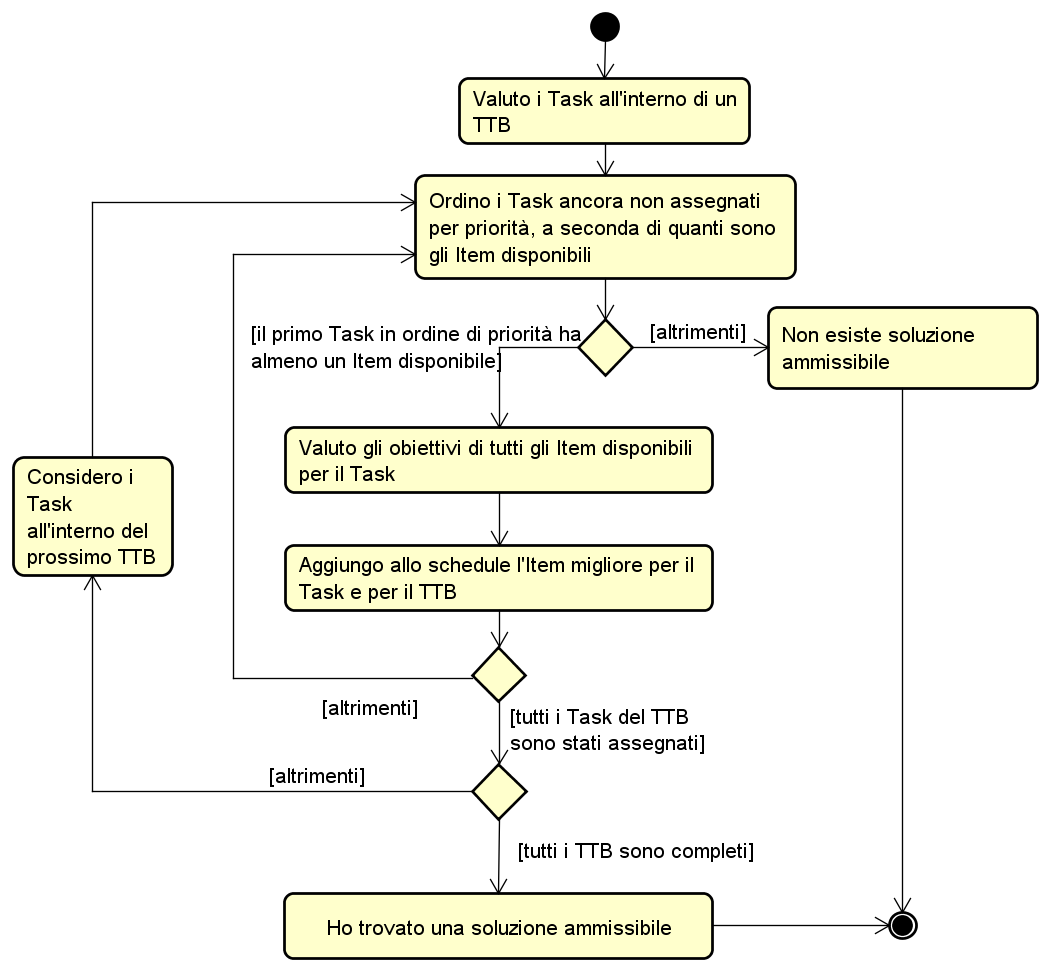
\includegraphics[width=16cm,keepaspectratio]{../immagini/algoritmo.png}
        \caption{Diagramma di attività per l'algoritmo greedy di risoluzione per i problemi di scheduling}
    \end{widepage}
\end{figure}
\FloatBarrier
\noindent
Si presenta tuttavia un problema: nel caso in cui gli \items\ non siano abbastanza da coprire tutti i \task\ durante i \ttb, questo algoritmo si blocca e non produce alcuno scheduling. Sapendo che tramite l'euristica si vuole creare uno scheduling iniziale da ottimizzare poi tramite metodi metaeuristici, il non riuscire a produrre uno scheduling iniziale potrebbe limitare l'efficacia delle stesse metaeuristiche. \\
\\
Nel paper \cite{paper:dummy}, per arrivare sempre a una soluzione ammissibile viene introdotto un \emph{\gls{dummy}}\glsfirstoccur
, che viene poi eliminato tramite la Neighborhood Search (metaeuristica). \\
\\
L'algoritmo di risoluzione implementato viene quindi lievemente modificato, sostituendo al secondo punto ``Se esiste un \task\ con nessun \items\ disponibile per la schedulazione, il \task\ viene assegnato al Dummy Worker''. Il risultante algoritmo è schematizzato in \hyperref[fig32]{Figura 3.2}.
\begin{figure}[!h]
    \label{fig32}
    \begin{widepage}
        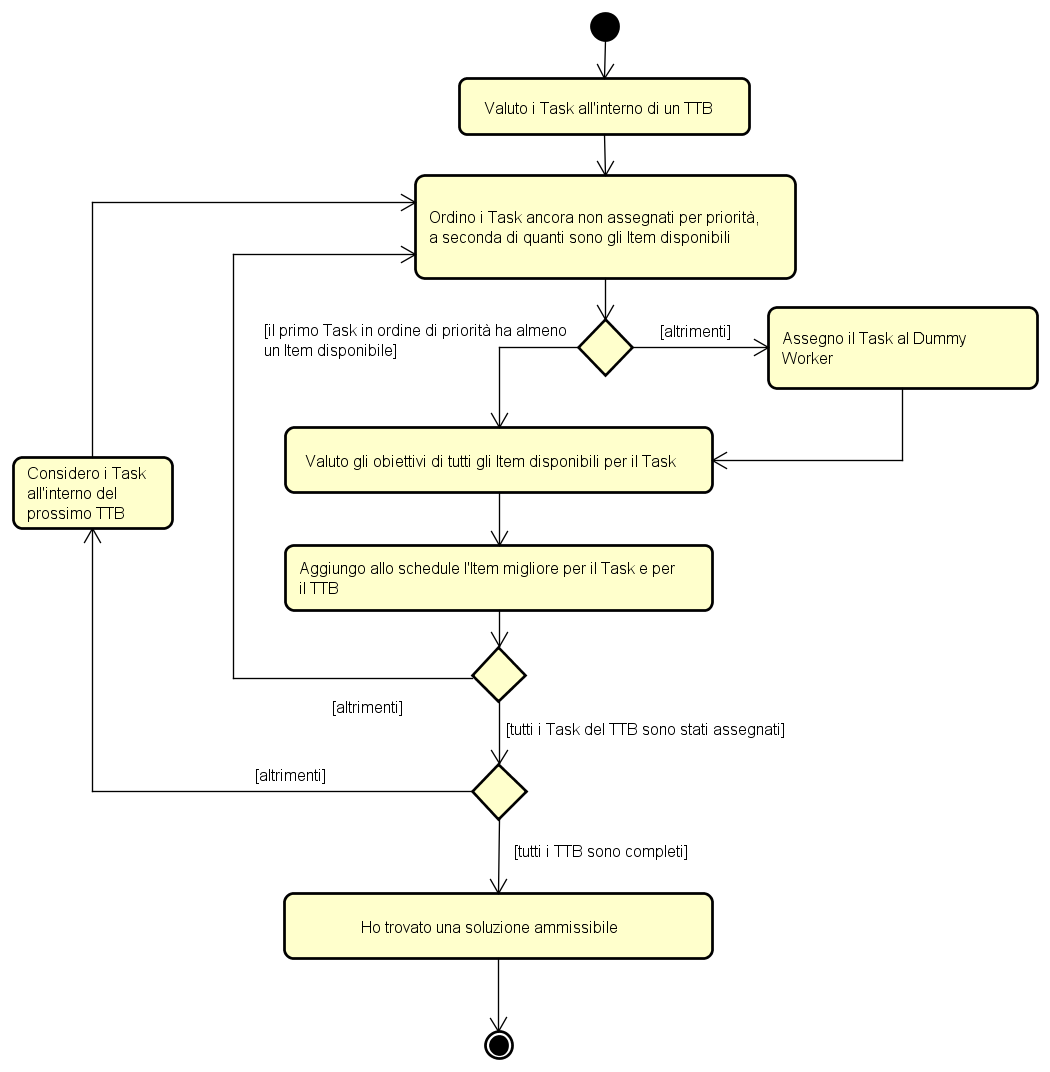
\includegraphics[width=16cm,keepaspectratio]{../immagini/algoritmo_dummy.png}
        \caption{Diagramma di attività per l'algoritmo greedy di risoluzione per i problemi di scheduling con aggiunta di Dummy Worker}
    \end{widepage}
\end{figure}             % Kick-Off
% !TEX encoding = UTF-8
% !TEX TS-program = pdflatex
% !TEX root = ../tesi.tex

%**************************************************************
\chapter{Analisi dei requisiti}
\label{cap:analisi-requisiti}
%**************************************************************

\intro{In questo capitolo vengono definite con precisione le funzionalità del software che è stato prodotto durante lo stage. Viene presentata l'analisi dei requisiti svolta per il progetto, approfondita con i diagrammi dei casi d'uso.}\\

\section{Casi d'uso}
I diagrammi dei casi d'uso (in inglese, \textit{Use Case Diagram}) sono diagrammi di tipo \gls{umlg} che servono a descrivere le interazioni fra il sistema software e gli utenti che lo utilizzano, mostrando l'insieme funzionalità esposte dal sistema dal punto di vista degli utenti. \\
Poiché lo stage era incentrato sull'estensione del framework e lo sviluppo di un algoritmo euristico per la risoluzione dei problemi di scheduling, la prima parte del progetto non necessitava di esporre funzionalità all'utente. D'altro canto, una volta sviluppata l'applicazione per risolvere il problema specifico del casinò, avrei dovuto garantire dei servizi minimi all'utente per inserire l'input (informazioni circa le postazioni, i lavoratori, i turni, etc...) e mostrare l'output (lo scheduling prodotto). \\
Per questo motivo i diagrammi dei casi d'uso risultano minimali e in numero ridotto.\\
\\
Ogni caso d'uso è classificato secondo la seguente convenzione:
\begin{center}
    UC[Codice padre]*.[Codice identificativo]
\end{center}

\begin{itemize}
    \item \textbf{Codice padre}: \MakeUppercase{} il codice identificativo del caso d'uso generico che ha generato il caso d'uso in esame. Se il caso d'uso non è stato generato da altri, va tralasciato;
    \item \textbf{Codice identificativo}: Identifica univocamente il caso d'uso. \MakeUppercase{è} un codice composto da sole cifre. 
\end{itemize}
\noindent
Alcuni casi d'uso possono essere associati ad un diagramma dei casi d'uso riportante lo stesso titolo e codice.
\clearpage
\subsection{Diagrammi dei casi d'uso}
\begin{figure}[!h]
    \begin{widepage}
        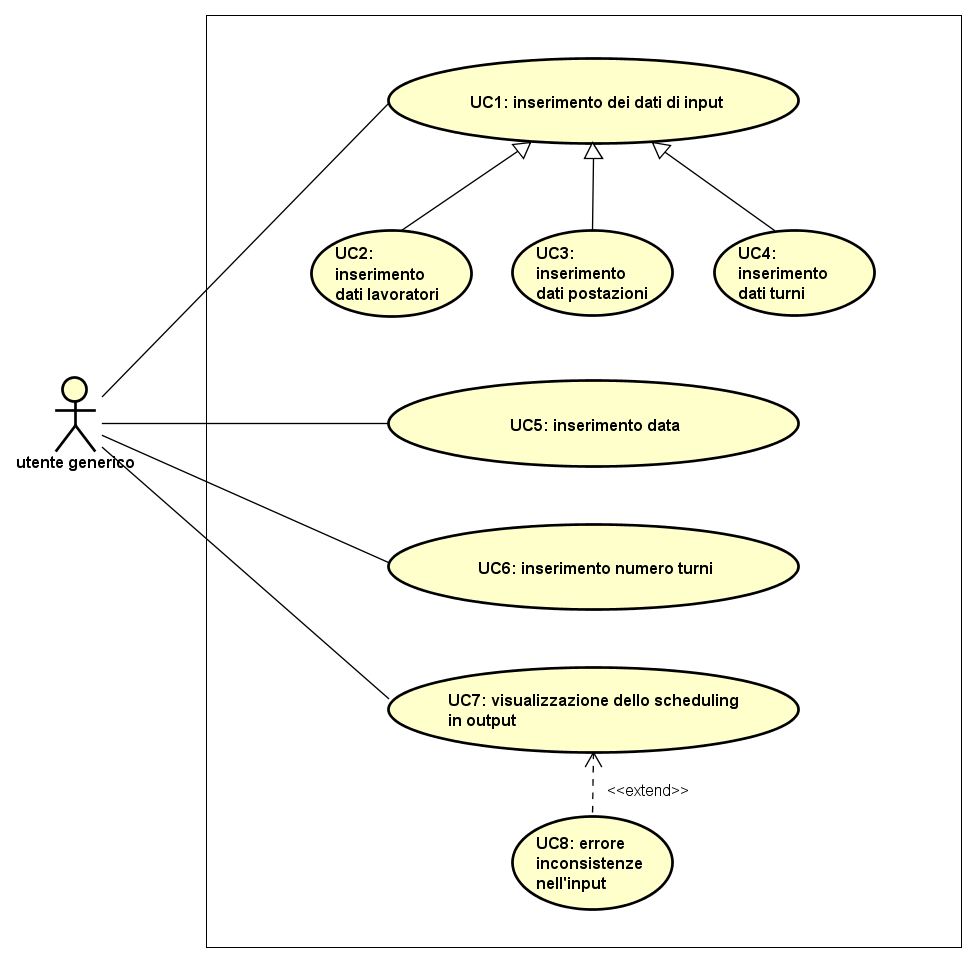
\includegraphics[width=17cm,keepaspectratio]{../immagini/usecase/System.png}
        \caption{Diagramma dei casi d'uso ad alto livello}
    \end{widepage}
\end{figure}
\clearpage
\subsection{UC1: Inserimento dei dati di input}
\label{UC1}
\begin{itemize}
    \item \textbf{Attori}: utente generico;
    \item \textbf{Descrizione}: l'utente inserisce i dati in input al programma per realizzare uno scheduling.
    \item \textbf{Generalizzazioni}: l'utente inserisce i dati in input al programma per realizzare uno scheduling riguardati i lavoratori (UC2), le postazioni (UC3), i turni (UC4).
\end{itemize}

\subsection{UC2: Inserimento dati lavoratori}
\label{UC2}
\begin{figure}[!h]
    \begin{widepage}
    \def\svgwidth{\columnwidth}
    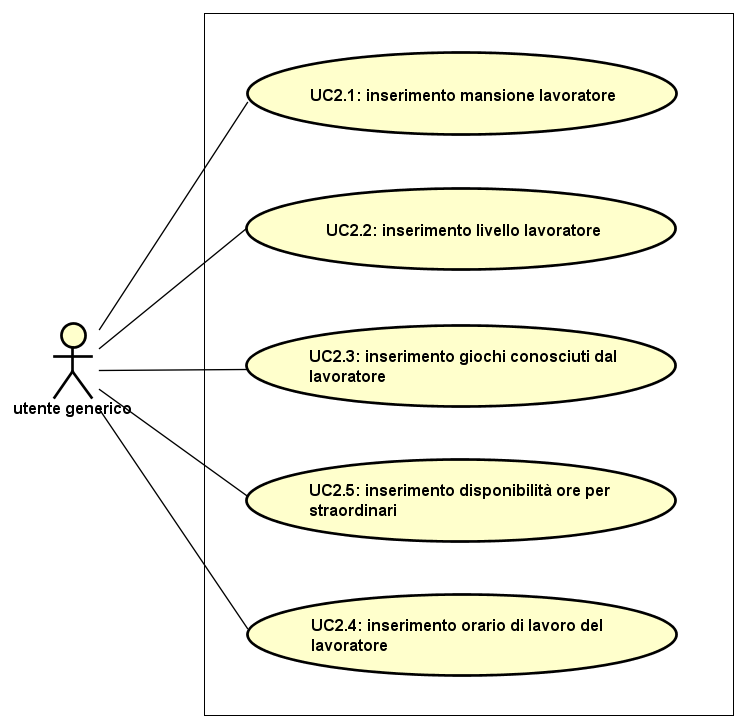
\includegraphics[width=14.9cm,keepaspectratio]{../immagini/usecase/UC2.png}
    \caption{UC2: Inserimento dati lavoratori}
    \end{widepage}
\end{figure}
\clearpage
\begin{itemize}
    \item \textbf{Attori}: utente generico;
    \item \textbf{Descrizione}: l'utente inserisce i dati in input al programma per realizzare uno scheduling riguardanti i lavoratori.
\end{itemize}
\paragraph{UC2.1: Inserimento mansione lavoratore}
\begin{itemize}
    \item \textbf{Attori}: utente generico;
    \item \textbf{Descrizione}: l'utente inserisce i dati in input al programma circa la mansione del lavoratore (dealer, dealer-inspector, inspector).
\end{itemize}
\paragraph{UC2.2: Inserimento livello lavoratore}
\begin{itemize}
    \item \textbf{Attori}: utente generico;
    \item \textbf{Descrizione}: l'utente inserisce i dati in input al programma circa il livello del lavoratore (dealer: 1-8, dealer-inspector: 3, inspector: 1-3).
\end{itemize}
\paragraph{UC2.3: Inserimento giochi conosciuti dal lavoratore}
\begin{itemize}
    \item \textbf{Attori}: utente generico;
    \item \textbf{Descrizione}: l'utente inserisce i dati in input al programma circa i giochi conosciuti dal lavoratore.
\end{itemize}
\paragraph{UC2.4: Inserimento orario di lavoro del lavoratore}
\begin{itemize}
    \item \textbf{Attori}: utente generico;
    \item \textbf{Descrizione}: l'utente inserisce i dati in input al programma circa l'orario di lavoro del giocatore (ora di inizio, ora di fine).
\end{itemize}
\paragraph{UC2.5: Inserimento disponibilità ore per straordinari}
\begin{itemize}
    \item \textbf{Attori}: utente generico;
    \item \textbf{Descrizione}: l'utente inserisce i dati in input al programma circa la disponibilità a svolgere straordinari (ore).
\end{itemize}
\clearpage
\subsection{UC3: Inserimento dati postazioni}
\label{UC3}
\begin{figure}[!h]
    \def\svgwidth{\columnwidth}
    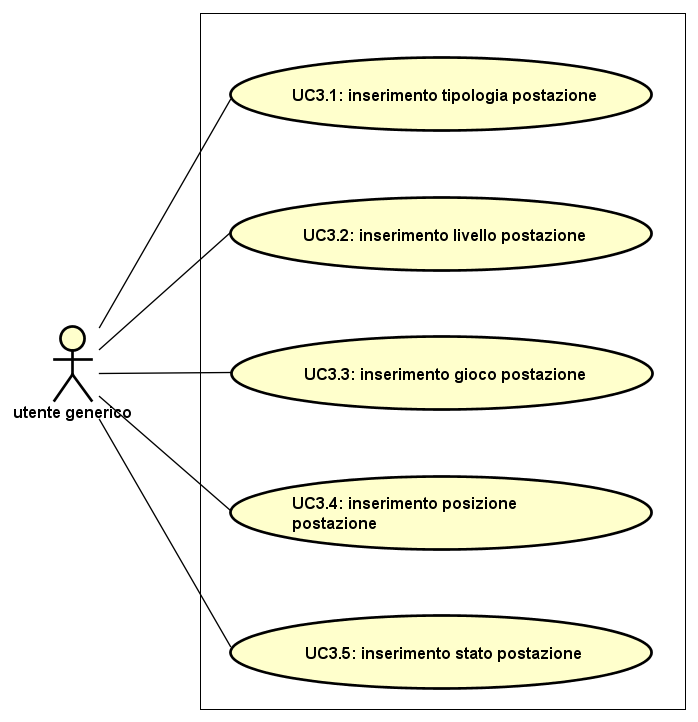
\includegraphics[width=\textwidth]{../immagini/usecase/UC3.png}
    \caption{UC3: Inserimento dati postazioni}
\end{figure}
\FloatBarrier
\noindent
\begin{itemize}
    \item \textbf{Attori}: utente generico;
    \item \textbf{Descrizione}: l'utente inserisce i dati in input al programma per realizzare uno scheduling riguardanti le postazioni.
\end{itemize}
\paragraph{UC3.1: Inserimento tipologia postazione}
\begin{itemize}
    \item \textbf{Attori}: utente generico;
    \item \textbf{Descrizione}: l'utente inserisce i dati in input al programma circa la tipologia della postazione (tavolo, pit).
\end{itemize}
\paragraph{UC3.2: Inserimento livello postazione}
\begin{itemize}
    \item \textbf{Attori}: utente generico;
    \item \textbf{Descrizione}: l'utente inserisce i dati in input al programma circa il livello della postazione (tavoli: 1-8, pit: 1-3).
\end{itemize}
\paragraph{UC3.3: Inserimento gioco postazione}
\begin{itemize}
    \item \textbf{Attori}: utente generico;
    \item \textbf{Descrizione}: l'utente inserisce i dati in input al programma circa il gioco che si gioca nella postazione.
\end{itemize}
\paragraph{UC3.4: Inserimento posizione postazione}
\begin{itemize}
    \item \textbf{Attori}: utente generico;
    \item \textbf{Descrizione}: l'utente inserisce i dati in input al programma circa la posizione che si assume lavorando nella postazione (seduta, in piedi).
\end{itemize}
\paragraph{UC3.5: Inserimento stato}
\begin{itemize}
    \item \textbf{Attori}: utente generico;
    \item \textbf{Descrizione}: l'utente inserisce i dati in input al programma circa lo stato della postazione (aperta, chiusa).
\end{itemize}
\subsection{UC4: Inserimento dati turni}
\label{UC4}
\begin{figure}[!h]
    \def\svgwidth{\columnwidth}
    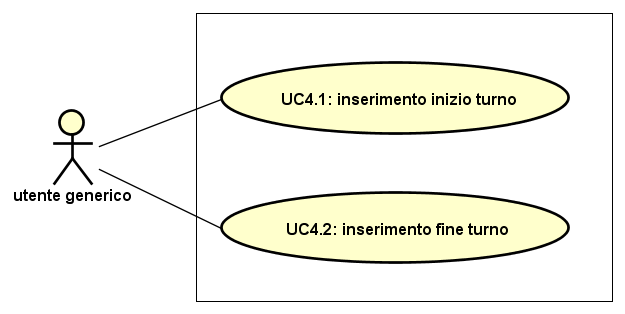
\includegraphics[width=\textwidth]{../immagini/usecase/UC4.png}
    \caption{UC4: Inserimento dati turni}
\end{figure}
\FloatBarrier
\noindent
\begin{itemize}
    \item \textbf{Attori}: utente generico;
    \item \textbf{Descrizione}: l'utente inserisce i dati in input al programma per realizzare uno scheduling riguardanti i turni.
\end{itemize}
\paragraph{UC4.1: Inserimento inizio turno}
\begin{itemize}
\item \textbf{Attori}: utente generico;
\item \textbf{Descrizione}: l'utente inserisce i dati in input al programma circa l'ora di inizio di un turno.
\end{itemize}
\paragraph{UC4.2: Inserimento fine turno}
\begin{itemize}
\item \textbf{Attori}: utente generico;
\item \textbf{Descrizione}: l'utente inserisce i dati in input al programma circa l'ora di fine di un turno.
\end{itemize}

\subsection{UC5: Inserimento data}
\label{UC5}
\begin{itemize}
    \item \textbf{Attori}: utente generico;
    \item \textbf{Descrizione}: l'utente inserisce la data per la quale vuole trovare uno scheduling (importante perché gli orari del personale possono variare di data in data).
    \item \textbf{Scenario alternativo}: se l'utente non inserisce una data, viene trovato lo scheduling per il giorno corrente.
\end{itemize}

\subsection{UC6: Inserimento numero turni}
\label{UC6}
\begin{itemize}
    \item \textbf{Attori}: utente generico;
    \item \textbf{Descrizione}: l'utente inserisce il numero di turni per il quale vuole trovare uno scheduling.
    \item \textbf{Scenario alternativo}: se l'utente non inserisce un numero, viene trovato lo scheduling per tutti i turni.
\end{itemize}

\subsection{UC7: Visualizzazione dello scheduling in output}
\label{UC7}
\begin{itemize}
    \item \textbf{Attori}: utente generico;
    \item \textbf{Descrizione}: l'utente visualizza l'output del programma (soluzione ammissibile o non).
    \item \textbf{Estensioni}: non c'è output perché è stato commesso un errore di inserimento dei dati.
\end{itemize}
\clearpage
%***********************************************************************
\section{Tracciamento dei requisiti}

Da un'attenta analisi dei requisiti e degli use case effettuata sul progetto è stata stilata la tabella che traccia i requisiti in rapporto agli use case.\\
Sono stati individuati diversi tipi di requisiti e si è quindi fatto utilizzo di un codice identificativo per distinguerli.\\
Il codice dei requisiti è così strutturato R(F/Q/V)(N/D/O) dove:
\begin{enumerate}
	\item[R =] requisito
    \item[F =] funzionale
    \item[Q =] qualitativo
    \item[V =] di vincolo
    \item[N =] obbligatorio (necessario)
    \item[D =] desiderabile
    \item[Z =] opzionale
\end{enumerate}
Nelle tabelle \ref{tab:requisiti-funzionali}, \ref{tab:requisiti-qualitativi} e \ref{tab:requisiti-vincolo} sono riassunti i requisiti e il loro tracciamento con gli use case delineati in fase di analisi.

\newpage

\begin{table}%
\caption{Tabella del tracciamento dei requisti funzionali}
\label{tab:requisiti-funzionali}
\begin{tabularx}{\textwidth}{lXl}
\hline\hline
\textbf{Requisito} & \textbf{Descrizione} & \textbf{Use Case}\\
\hline
RFN-1     & L'interfaccia permette di configurare il tipo di sonde del test & UC1 \\
\hline
\end{tabularx}
\end{table}%

\begin{table}%
\caption{Tabella del tracciamento dei requisiti qualitativi}
\label{tab:requisiti-qualitativi}
\begin{tabularx}{\textwidth}{lXl}
\hline\hline
\textbf{Requisito} & \textbf{Descrizione} & \textbf{Use Case}\\
\hline
RQD-1    & Le prestazioni del simulatore hardware deve garantire la giusta esecuzione dei test e non la generazione di falsi negativi & - \\
\hline
\end{tabularx}
\end{table}%

\begin{table}%
\caption{Tabella del tracciamento dei requisiti di vincolo}
\label{tab:requisiti-vincolo}
\begin{tabularx}{\textwidth}{lXl}
\hline\hline
\textbf{Requisito} & \textbf{Descrizione} & \textbf{Use Case}\\
\hline
RVO-1    & La libreria per l'esecuzione dei test automatici deve essere riutilizzabile & - \\
\hline
\end{tabularx}
\end{table}%             % Concept Preview
% !TEX encoding = UTF-8
% !TEX TS-program = pdflatex
% !TEX root = ../tesi.tex

%**************************************************************
\chapter{Progettazione e codifica}
\label{cap:progettazione-codifica}
%**************************************************************

\intro{ presenta la progettazione svolta per il progetto, approfondita con diagrammi \emph{UML}\glsfirstoccur,
    e ne descrive la fase di codifica.}\\

%**************************************************************
\section{Tecnologie e strumenti}
\label{sec:tecnologie-strumenti}

Di seguito viene data una panoramica delle tecnologie e strumenti utilizzati.

\subsection*{Tecnologia 1}
Descrizione Tecnologia 1.

\subsection*{Tecnologia 2}
Descrizione Tecnologia 2

%**************************************************************
\section{Progettazione}
\label{sec:progettazione}

\subsubsection{Namespace 1} %**************************
Descrizione namespace 1.

\begin{namespacedesc}
    \classdesc{Classe 1}{Descrizione classe 1}
    \classdesc{Classe 2}{Descrizione classe 2}
\end{namespacedesc}


%**************************************************************
\section{Design Pattern utilizzati}

%**************************************************************
\section{Codifica}
             % Product Prototype
% !TEX encoding = UTF-8
% !TEX TS-program = pdflatex
% !TEX root = ../tesi.tex

%**************************************************************
\chapter{Verifica e validazione}
\label{cap:verifica-validazione}
%**************************************************************
\intro{In questo capitolo viene approfondito il periodo di verifica e test, durante il quale sono emerse alcune difficoltà che hanno richiesto un tempo maggiore del previsto per la risoluzione. Viene qui presentata la modalità di risoluzione di queste difficoltà, unita ai risultati ottenuti durante i test e i dati emersi dalle analisi dei risultati.}
%**************************************************************
\section{Generazione degli input}
Una volta accertatami che il comportamento della \emph{\gls{bus-logic}}\glsfirstoccur\ del software prodotto fosse corretto su piccoli input di prova, si è presentato il problema di testare l'applicazione su istanze di input più grandi e con più variabili. Da piano di lavoro, il tempo previsto per verifica, testing e analisi dei risultati era stabilito di 20 ore; tuttavia, è stato da subito chiaro che il processo di verifica sarebbe stato più complicato del previsto.\\
Per eseguire test significativi in serie, era infatti necessario poter produrre automaticamente degli input su cui il software potesse elaborare per produrre scheduling: è stata quindi estesa la classe \texttt{Excel} per poter andare a modificare in scrittura i fogli xls di input. In un primo momento, si è provato a generare degli input randomici, ma tale soluzione si è rivelata problematica per due motivi: in primo luogo, gli input randomici non producevano praticamente mai delle soluzioni ammissibili in quanto spesso ci si trovava con un sbilanciamento postazioni/lavoratori; in secondo luogo, anche quando veniva (raramente) prodotta una soluzione ammissibile, tale soluzione non poteva essere rappresentativa di un buono scheduling in quanto non era sensata. Il problema principale da risolvere è quindi diventato \textit{come} generare degli input il più possibile vicini alla realtà che potessero produrre degli scheduling da analizzare.\\
Il problema è stato esposto al tutor aziendale, che ha approvato la modifica al piano di lavoro assegnando più ore alla verifica e al testing, tagliando su attività per il raggiungimento di requisiti desiderabili e opzionali, ritenendo più importante poter testare il software in maniera corretta e approfondita. \\
\\
Secondo le informazioni fornite dal casinò, gli input per essere realistici dovevano:
\begin{itemize}
    \item comprendere circa 30 postazioni aperte contemporaneamente, per un totale di 40 lavoratori attivi. Il totale dei lavori, per garantire quindi uno scheduling fair e rispettoso delle pause e dei vincoli previsti, doveva ammontare a circa il 33\%\ in più rispetto al numero di postazioni.
    \item di tutte le postazioni aperte, alla maggior parte viene assegnato un livello basso e giochi comunemente conosciuti dai lavoratori, mentre le postazioni che richiedono un livello alto o giochi poco conosciuti sono meno.
    \item il livello dei lavoratori dipende dal tempo passato all'interno del casinò e dalle loro abilità, di conseguenze la maggior parte dei lavoratori è di livello intermedio, mentre sono pochi quelli di livello molto alto e molto basso.
    \item i giochi conosciuti dai lavoratori dipende dal loro livello: più un dealer è di livello alto, più giochi conosce; per quanto riguarda inspector e dealer-inspector, essi conoscono praticamente tutti i giochi.
\end{itemize}
Sulle basi di queste informazioni, è stato possibile produrre un modello probabilistico che descrivesse una situazione reale e progettare una nuova classe, \texttt{Test}, che generasse automaticamente ad ogni \textit{run} dell'algoritmo un set di input secondo il modello definito.

\subsection{Modello probabilistico}

Tutti i grafici presenti in questa sezione sono stati prodotti sul sito di Wolfram Alpha\footcite{https://www.wolframalpha.com/examples/StatisticalDistributions.html}.
    \paragraph{Numero di postazioni} Ipotizzando che il numero di postazioni aperte contemporaneamente sia circa 30, genero il numero di postazioni tramite una distribuzione normale $\mathcal{N}(\mu;\sigma \ap{2})$ con:
    \begin{itemize}
        \item tavoli: $\mu = 20$, $\sigma \ap{2} = \frac{\mu}{5}$
        \item pit: $\frac{tavoli}{3}$
    \end{itemize}

    \begin{figure}[!htb]
    \begin{widepage}
    \centering
    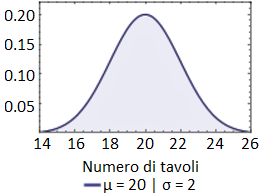
\includegraphics[width=.49\textwidth]{../immagini/gauss_tavoli_w.png}\hfil
    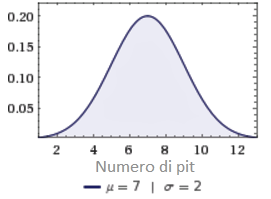
\includegraphics[width=.49\textwidth]{../immagini/gauss_pit_w.png}
    \caption{Distribuzioni normali per il numero di postazioni}
    \end{widepage}
    \end{figure}
\clearpage
    \paragraph{Costruzione delle postazioni} Ipotizzando che le postazioni che richiedono un livello alto sono poche e viceversa, genero i livelli delle postazioni L\ped{t} con una distribuzione discreta uniforme $\mathcal{U}(\mathcal{S})$ dove \[\mathcal{S} = \{ \alpha + i*\beta \text{ t.c. } i \in \{0,2,...,n\} \} \] ovvero i cui elementi sono i progressione aritmetica con $\alpha = 1$, $\beta = 1$ e:
    \begin{itemize}
        \item per i tavoli (8 livelli): $n = 7$
        \item per i pit (3 livelli): $n = 2$
    \end{itemize}
    \begin{figure}[!htb]
        \begin{widepage}
            \centering
            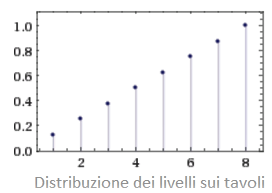
\includegraphics[width=.49\textwidth]{../immagini/discr_livelli_tavoli.png}\hfil
            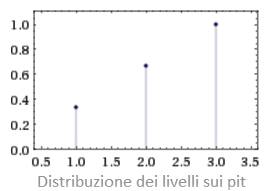
\includegraphics[width=.49\textwidth]{../immagini/discr_livelli_pit.png}
            \caption{Distribuzione discreta uniforme per i livelli delle postazioni}
        \end{widepage}
    \end{figure}
    \FloatBarrier
    \noindent
    Inoltre viene generato il gioco richiesto ad una certa postazione in modo che la frequenza del gioco base (//) sia doppia rispetto a quella di altri giochi (BJ e PG).\\
    Ad ogni postazione è richiesto un solo gioco.
    
    \begin{figure}[!htb]
        \begin{widepage}
            \centering
            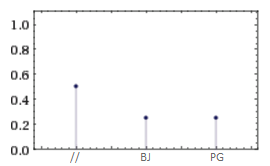
\includegraphics[width=.49\textwidth]{../immagini/distr_giochi_tavoli.png}
            \caption{Frequenza di estrazione dei giochi per ogni postazione}
        \end{widepage}
    \end{figure}%
    \clearpage
    \paragraph{Numero di lavoratori} Ipotizzando che il numero di lavoratori attivi contemporaneamente sia di circa il 33\% in più rispetto al numero di postazioni, genero il numero di lavoratori tramite una distribuzione normale $\mathcal{N}(\mu;\sigma \ap{2})$ con:
    \begin{itemize}
        \item dealer: $\mu = tavoli*1.6$, $\sigma \ap{2} = \frac{tavoli}{5}$
        \item inspector: $\mu = pit*1.6$, $\sigma \ap{2} = \frac{pit}{5}$
    \end{itemize}

    \begin{figure}[!htb]
        \begin{widepage}
        \centering
        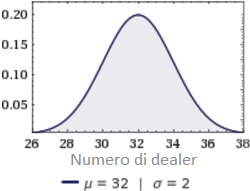
\includegraphics[width=.49\textwidth]{../immagini/gauss_dealer_w.png}\hfil
        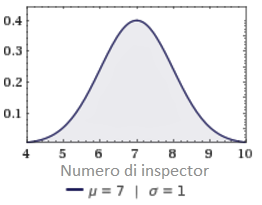
\includegraphics[width=.49\textwidth]{../immagini/gauss_inspector_w.png}
        \caption{Distribuzioni normali per il numero di lavoratori}
        \end{widepage}
    \end{figure}
    \FloatBarrier
    \noindent
    Da notare che il valor medio $\mu$ è stato fissato al 60\% in più rispetto al numero di postazioni, sarà poi compito dell'algoritmo andare ad ottimizzare il numero di lavoratori richiesti per riempire lo scheduling. \\
    \\
    Per quanto riguarda il numero di dealer-inspector, esso viene fissato a \[(tavoli + pit) * 1.6 - dealer - inspector\] per far sì che il numero di lavoratori attivi sia sempre esattamente il 60\% in più rispetto al numero di postazioni.
    \clearpage
    \paragraph{Costruzione dei lavoratori} Ipotizzando che il livello dei lavoratori dipenda solo dal tempo che hanno passato all'interno del casinò, generiamo i livelli dei lavoratori L\ped{w} tramite una distribuzione normale $\mathcal{N}(\mu;\sigma \ap{2})$ con:
    \begin{itemize}
        \item dealer: $\mu = 4.5$, $\sigma \ap{2} = \frac{\mu}{3.5}$
        \item inspector: $\mu = 2$, $\sigma \ap{2} = \frac{\mu}{1}$
    \end{itemize}
     \begin{figure}[!htb]
         \begin{widepage}
             \centering
             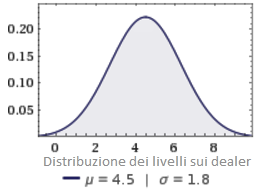
\includegraphics[width=.49\textwidth]{../immagini/livelli_dealer.png}\hfil
             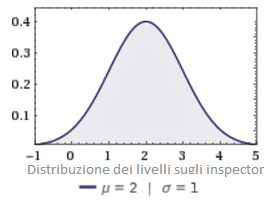
\includegraphics[width=.49\textwidth]{../immagini/livelli_insp.png}
             \caption{Distribuzioni normali per i livelli dei lavoratori di lavoratori}
         \end{widepage}
     \end{figure}
     \FloatBarrier
     \noindent
     Ipotizzando che la probabilità che un lavoratore conosca un gioco sia direttamente proporzionale al suo livello (più un lavoratore ha livello alto, più giochi conosce; tutti conoscono i giochi base //), generiamo i giochi che ogni lavoratore conosce con una distribuzione di Bernoulli $\mathcal{B}e(p)$ dove $p = 1 - \frac{livello}{10}$.
     \begin{figure}[!htb]
         \begin{widepage}
             \centering
             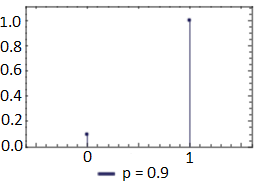
\includegraphics[width=.49\textwidth]{../immagini/livello_1.png}\hfil
             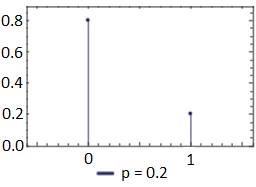
\includegraphics[width=.49\textwidth]{../immagini/livello_8.png}
             \caption{Probabilità che due lavoratori di livelli 1 (a sinistra) e 8 (a destra) conoscano un gioco (1) o meno (0)}
         \end{widepage}
     \end{figure}
 \clearpage
\subsection{Progettazione}
%**************************************************************
\section{Esiti dei test}             % Product Design Freeze e SOP
% !TEX encoding = UTF-8
% !TEX TS-program = pdflatex
% !TEX root = ../tesi.tex

%**************************************************************
\chapter{Conclusioni}
\label{cap:conclusioni}
%**************************************************************
\intro{ riporta le conclusioni oggettive e soggettive a cui si è giunti per il progetto.}
%**************************************************************
\section{Consuntivo finale}

%**************************************************************
\section{Raggiungimento degli obiettivi}

%**************************************************************
\section{Attualizzazione dei rischi}

%**************************************************************
\section{Conoscenze acquisite}

%**************************************************************
\section{Valutazione personale}
             % Conclusioni
%\appendix                               
%% !TEX encoding = UTF-8
% !TEX TS-program = pdflatex
% !TEX root = ../tesi.tex

%**************************************************************
\chapter{Appendice A}
%**************************************************************

\epigraph{Citazione}{Autore della citazione}



             % Appendice A

%**************************************************************
% Materiale finale
%**************************************************************
\backmatter
\printglossaries
% !TEX encoding = UTF-8
% !TEX TS-program = pdflatex
% !TEX root = ../tesi.tex

%**************************************************************
% Bibliografia
%**************************************************************

\cleardoublepage
\chapter{Bibliografia}

\nocite{*}
% Stampa i riferimenti bibliografici
\printbibliography[heading=subbibliography,title={Riferimenti bibliografici},type=book]

% Stampa i siti web consultati
\printbibliography[heading=subbibliography,title={Siti web consultati},type=online]
\end{document}